%%
% The BIThesis Template for Bachelor Graduation Thesis
%
% 北京理工大学毕业设计(论文)第二章节 —— 使用 XeLaTeX 编译
%
% Copyright 2020-2021 BITNP
%
% This work may be distributed and/or modified under the
% conditions of the LaTeX Project Public License, either version 1.3
% of this license or (at your option) any later version.
% The latest version of this license is in
%   http://www.latex-project.org/lppl.txt
% and version 1.3 or later is part of all distributions of LaTeX
% version 2005/12/01 or later.
%
% This work has the LPPL maintenance status `maintained'.
%
% The Current Maintainer of this work is Feng Kaiyu.
% 第四章

\chapter{环境搭建}

\section{软件环境}

\subsection{编译工具链}
step1.访问sifive官网,下载riscv gcc toolchain

\href{https://www.sifive.com/software}{https://www.sifive.com/software}

step2.找到Prebuilt RISC-V GCC Toolchain。根据开发环境选择对应的版本。

\begin{figure}[htbp]
    \vspace{13pt} % 调整图片与上文的垂直距离
    \centering
    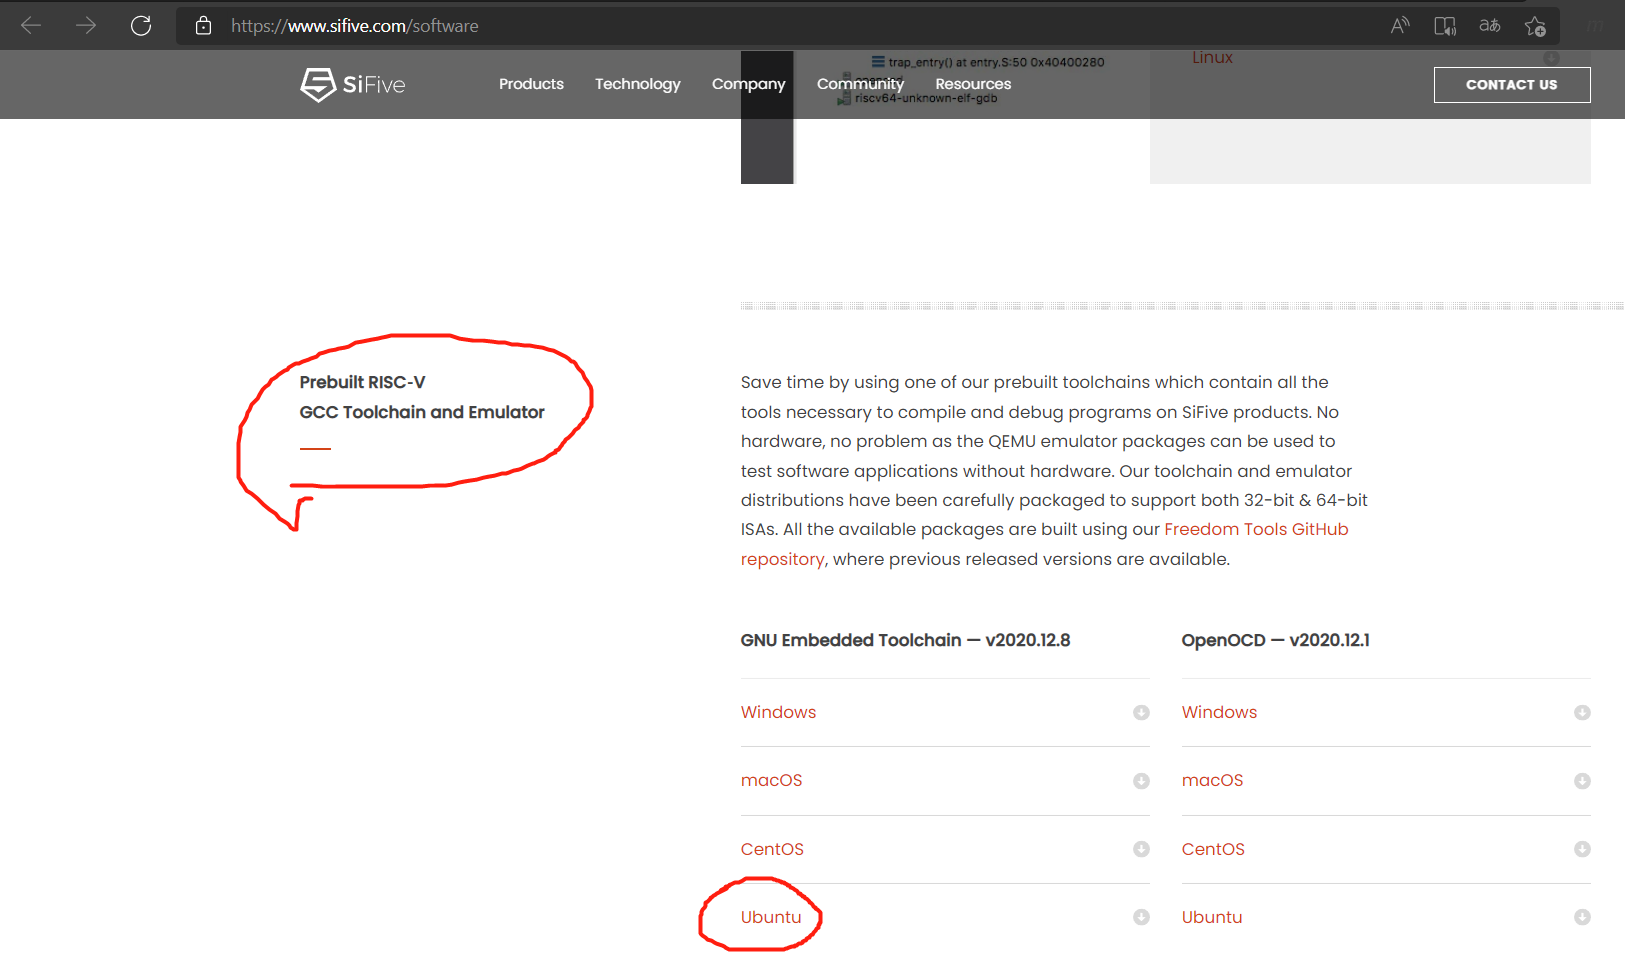
\includegraphics[width=0.9\textwidth]{images/toolchain.png}
    \caption{编译工具链列表}\label{编译工具链列表} % label 用来在文中索引
\end{figure}

step3.将下载好的tar.gz压缩包解压

\begin{lstlisting}[caption={解压命令}, label={lst:tar_command}]
    tar -zxvf $your_tar_gz
\end{lstlisting}

step4.配置环境变量。解压完成得到文件夹,进入文件夹里的bin目录,打开terminal,输入pwd获得当前路径。
复制获得的路径。将复制到的路径加入系统的PATH环境变量。

\begin{lstlisting}[caption={修改环境变量}, label={lst:change_env}]
    vim /etc/profile
    #添加以下两行到文件末尾
    export RISCV=$your_path
    export PATH=$PATH:$RISCV
\end{lstlisting}

\begin{figure}[htbp]
    \vspace{13pt} % 调整图片与上文的垂直距离
    \centering
    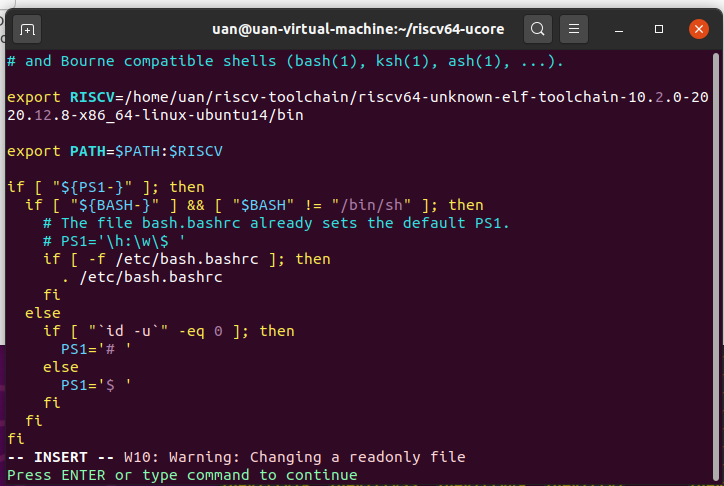
\includegraphics[width=0.9\textwidth]{images/env_path.png}
    \caption{配置环境变量}\label{配置环境变量} % label 用来在文中索引
\end{figure}

step5.加载环境变量文件

\begin{lstlisting}[caption={加载环境变量文件}, label={lst:load_env_profile}]
    source /etc/profile
\end{lstlisting}

step6.验证编译环境

在终端输入 riscv64-unknown-elf-gcc -v,如果出现以下内容,则编译环境配置成功。

\begin{lstlisting}[caption={验证编译环境}, label={lst:check_env}]
    Using built-in specs.
    ....
    gcc version 10.2.0 (SiFive GCC-Metal 10.2.0-2020.12.8) 
\end{lstlisting}

\subsection{代码准备}

step1.下载riscv64-pke-k210的代码库并查看所有分支

\begin{lstlisting}[caption={下载代码库}, label={lst:download_code}]
    git clone git@github.com:BITzga/riscv64-pke-k210.git
    git branch -a
\end{lstlisting}

step2.根据开发需求选择分支。

如下所示,k210前缀的代码分支是根据k210环境移植完成的代码。而其他普通分支则是PKE原先的代码。此时,根据开发需求使用git checkout命令选择分支即可。

\begin{lstlisting}[caption={分支列表}, label={lst:branch_list}]
    remotes/origin/k210/lab1_1_syscall
    remotes/origin/k210/lab1_2_exception
    remotes/origin/k210/lab1_3_irq
    remotes/origin/k210/lab2_1_pagetable
    remotes/origin/k210/lab2_2_allocatepage
    remotes/origin/k210/lab2_3_pagefault
    remotes/origin/k210/lab3_1_fork
    remotes/origin/k210/lab3_2_yield
    remotes/origin/k210/lab3_3_rrsched
    remotes/origin/lab1_1_syscall
    remotes/origin/lab1_2_exception
    remotes/origin/lab1_3_irq
    remotes/origin/lab2_1_pagetable
    remotes/origin/lab2_2_allocatepage
    remotes/origin/lab2_3_pagefault
    remotes/origin/lab3_1_fork
    remotes/origin/lab3_2_yield
    remotes/origin/lab3_3_rrsched
    remotes/origin/master
\end{lstlisting}


\subsection{编辑器、IDE选择}

\subsection{K210环境}

\begin{itemize}
    \item Python3环境
    
    由于烧录程序和串口调试工具都是使用Python3编写的。Python是解释型语言,所以我们需要安装Python3解释器。
    除此之外我们还需要安装Python包管理工具pip。

    \begin{lstlisting}[caption={安装Python3环境}, label={lst:install_python3}]
        sudo apt-get install python3
        sudo apt-get install python3-pip
    \end{lstlisting}

    \item 烧录工具
    我们编写好的程序,经过编译,变成bin文件,还需要烧录到K210上才能运行。而烧录需要借助烧录工具,这里我们使用了\href{https://github.com/BITzga/riscv64-pke-k210/blob/master/compile_tool/kflash.py}{K-Flash}。
    \item 串口调试工具
    内核在运行时,输出信息是通过串口输出的,我们需要一个串口调试工具来接收K210上的串口信息。这里我们需要安装并使用miniterm。

    \begin{lstlisting}[caption={安装miniterm}, label={lst:install_miniterm}]
        sudo apt-get install miniterm
    \end{lstlisting}

    \item RustSBI-K210支持包
    SBI是RISC-V的规范之一,它规定了监管者二进制(Supervisor Binary Interface)接口。
    RustSBI-K210是SBI标准的一种实现,它使用Rust语言进行编写,具有性能安全的特点。
    除此之外,RustSBI-K210还对K210板子提供了特殊的支持。它还可以在K210上作为我们内核程序的Bootloader。
    我们需要使用RustSBI-K210支持包来支持内核移植,这里我们需要在烧录内核时引入RustSBI-K210支持包。

    在这里,我们可以下载到RustSBI-K210的release版本

    \href{https://github.com/rustsbi/rustsbi-k210/releases}{https://github.com/rustsbi/rustsbi-k210/releases}
    
\end{itemize}

\section{硬件环境}

\subsection{K210硬件要求}

硬件环境较为简单,我们只需要一块具有串口功能的K210板子和一根数据线即可。

